\documentclass[10pt]{article}
\usepackage[fontsize=15pt]{fontsize}
\usepackage[utf8]{inputenc}
\usepackage[T2A]{fontenc}
\usepackage{amssymb}
\usepackage[letterpaper,top=2cm,bottom=2cm,left=3cm,right=3cm,marginparwidth=1.75cm]{geometry}
\usepackage{amsmath}
\usepackage{graphicx}
\usepackage[colorlinks=true, allcolors=blue]{hyperref}
\usepackage{pgfplots}
\pgfplotsset{compat=1.17}
\usepackage{titlesec}

\titleformat{\section}[display]{\centering\Large\bfseries}{\thesection}{1em}{}
\setcounter{page}{96}

\newcommand\textline[4][t]{%
  \par\smallskip\noindent\parbox[#1]{.333\textwidth}{\raggedright\texttt{+}#2}%
  \parbox[#1]{.333\textwidth}{\centering#3}%
  \parbox[#1]{.333\textwidth}{\raggedleft\texttt{#4}}\par\smallskip%
}


\begin{document}

Подставив в уравнение окружностн, полуиим уравнеиие эллипса $\frac{x^2}{a^2}+\frac{y^2}{b^2}=1$. Пусть окружиость задаиа в параметрической форме: $x=a \cos t, \quad y=a \sin t$ $\left(t \in[0,2 \pi)\right.$ ). Из (11.18) находим $X=a \cos t, Y=\frac{b}{a} y=$ $=b \cos t(t \in[0,2 \pi))$. Поэтому параметрическое уравнение эллипса с полуосями $a$ и $b$ имеют вид
\[
\left\{\begin{array}{l}
x=a \cos t \\
y=b \sin t
\end{array}\right\}(0 \leqslant t<2 \pi) .\tag{11.19}\label{myeq}
\]


В следующей лекции мы изучнм гиперболу и параболу.
\section*{Лекция 12}
\subsection{ГИПЕРБОЛА, ЕЕ СВОЙСТВА И ФОРМА.\\ПАРАБОЛА; ЕЕ СВОЙСТВА И ФОРМА.\\ПОЛЯРНОЕ УРАВНЕНИЕ ЭЛЛИПСА, ГИПЕРБОЛЫ И ПАРАБОЛЫ.\\УСЛОВИЯ КАСАНИЯ ПРЯМОЙ И КРИВОЙ ВТОРОГО ПОРЯДКА}
Перейдем к установлению геометрических свойств и формы гинерболы

\[
\frac{x^2}{a^2}-\frac{y^2}{b^2}=1(a, b>0) .\tag{12.1}\label{myeq}
\]


Введем параметр $c>0$ с помощью равенства $c^2=a^2+b^2$, так что $c>a$, и рассмотрим на оси $O x$ две точки $F_1(-c ; 0)$ и $F_2(c ; 0)$, которые назовем левым и правьм фокусами гиперболы. Вычнслим фокальные расстояния $\left|\overrightarrow{F_1 M}\right|,\left|\overrightarrow{F_2 M}\right|$ до произвольиой точки гиперболы $M(x ; y):\left|\overrightarrow{F_1 \vec{M}}\right|=r_1=\sqrt{(x+c)^2+y^2},\left|\overrightarrow{F_2 M}\right|=r_2=$ $=\sqrt{(x-c)^2+y^2}$. Из (12.1) находнм $y^2=\frac{c^2}{a^2} x^2-x^2-$ $-c^2+a^2$ и подставляем в выражения для $r_1$ и $r_2$. Имеем
\newpage
\[
\left.\begin{array}{l}
r_1=\sqrt{\left(a+\frac{c}{a} x\right)^2}=|a+e x| \\
r_2=\sqrt{\left(a-\frac{c}{a} x\right)^2}=|a-e x|
\end{array}\right\},\tag{12.2}\label{myeq}
\]

где $e=\frac{c}{a}$ - параметр, называемый эксцентриситетом гиперболы. Заметим, что для гилерболы $e>1$, так как $c>a$.

Исследуем различиые возможности, представляемые равеиствами (12.2). Из (12.1) следует $\frac{x^2}{a^2} \geqslant 1$, т. е. $|x| \geqslant a$. Поэтому в зависимости от того, лежит ли $M(x ; y)$ в правои полуплоскости $(x>0)$ или в левои $(x<0)$, выражеиия для (12.2) разлнчиые,

Если $x>0$, то $a+e x>0$ и $a-e x<0$, так как $e>\mathrm{I}, \boldsymbol{x}>a, e x>a$. Поэтому в правой полуплоскости выполнеио
\[
r_1=a+e x, \quad r_2=-a+e x .\tag{12.3}\label{myeq}
\]

Если $x<0$, то $a+e x<0$, так как $|e x|>a$, и $a-e x>0$. Позтому в левои полуплоскости выполнено
\[
r_1 = -a-e x, r_2=a-e x .\tag{12.4}\label{myeq}
\]

Из этих рассуждений вытекает, что типербола состоит из двух симметричных ветвей, расположеииых соответствеино в правой и левой полуплоскостях. Из (12.3), (12.4) для обенх ветвей выводим инвариантиое равенство
\[
\left|r_1-r_2\right|=2 a . \tag{12.5}\label{myeq}
\]

На основании (12.5) можно дать новое определение гиперболы как ГМТ плоскости, модуль разности расстояний от которых до двух фиксированкых точек $F_1 . F_1$, называемых фокусами гиперболы, есть величина постоянная (не равная нулю и меньшая расстояния между фокусами).

При устяновлении формы гиперболы отметим, что оси $O x$ и $О y$ являются осями симметрии, а их пересечение - центром симметрии (центр гиперболы). Поскольку $\frac{x^2}{a^2}.>1(|x| \geqslant a)$, то ветви гиперболы лежат

\newpage

на плоскости вне полосы $-a<x<a$, Точки пересечёния ветвей с осью $О x\left(y=0, A_1(-a ; 0), A_2(a ; 0)\right.$ ) называются вершинами гиперболы. Для гиперболы, заданной уравнением (12.1), ось $O x$ вазывается действительной осью гиперболы, а ось $О у$ - мнимой осью гиперболы (пересечения нет из-за равенства $-\frac{y^2}{b^2}=1$ ). В силу симметрий достаточно исследовать форму гиперболы в первой четверти, $y=\frac{b}{a} \sqrt{x^2-a^2}$, а затем распространить ва всю плоскость. Наряду с указанной ветвью гиперболы целесообразно рассмотреть луч, исходящий из начала координат, с уравненнем $\boldsymbol{r}=\frac{b}{a} x$

Пусть $M$-точка гиперболы с абсциссой $x, N-$ точка указанной прямой с той же абсциссой. Для разности ординат имеем
$$
Y-y=\frac{b}{a}\left(x-\sqrt{x^2-a^2}\right) .
$$

При неограниченном возрастании $\boldsymbol{x}$ данная разность монотонно стремится к нулю, так как
$$
\begin{gathered}
\lim _{x \rightarrow \infty}(Y-y)=\frac{b}{a} \lim _{x \rightarrow \infty}\left(x-\sqrt{x^2-a^2}\right)= \\
=\frac{b}{a} \lim _{x \rightarrow \infty} \frac{x^2-x^2+a^2}{\left(x+\sqrt{x^2-a^2}\right)}=0 .
\end{gathered}
$$

Поэтому прямые $y= \pm \frac{b}{a} x$ являются асимптотами гиперболы $\frac{x^2}{a^2}-\frac{y^2}{b^2}=1$. Для построения асимптот строим прямоугольннк со сторонамн $x= \pm a, y= \pm b$. Асимптоты - прямые, содержащие диагонали прямоугольника. При построенни гиперболы удобно построить сначала асимптоты, а затем ветви гиперболы (рис. 25а).

Для гиперболы вводятся две прямые, перпендикулярные к оси $O x$, с уравнениями $\left(x= \pm \frac{a}{e}\right.$ ) и называемые директрисами гиперболы. В силу неравенства $e>1$ директрнсы лежат между вершннаин гиперболы.

\newpage

\begin{center}
    a)\\
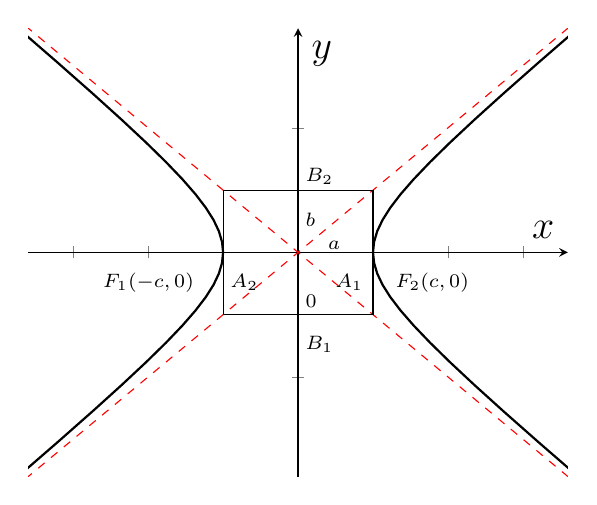
\begin{tikzpicture}[
every label/.style = {font=\tiny, inner sep=2pt, anchor=west},
        dot/.style = {circle, fill, inner sep = 1pt}
                        ]
    \begin{axis}[
        axis lines=middle,
        xlabel=$x$,
        ylabel=$y$,
        xmin=-3, xmax=3,
        ymin=-3, ymax=3,
        yticklabel=\\, xticklabel=\\,
        enlargelimits]
        \addplot [thick,domain=-2:2] ({cosh(x)}, {sinh(x)});
        \addplot [thick,domain=-2:2] ({-cosh(x)}, {sinh(x)});
        \addplot[red,dashed] expression {x};
        \addplot[red,dashed] expression {-x};
        \addplot[solid, draw = black] coordinates {(-1,1) (1,1) (1,-1) (-1,-1) (-1,1)};
        \node[label=135:{0}] at (0.2,-1) {};
        \node[label=135:{$B_1$}] at (0.2,-1.7) {};
        \node[label=135:{$B_2$}] at (0.2,1) {};
        \node[label=135:{$A_1$}] at (0.6,-0.7) {};
        \node[label=135:{$A_2$}] at (-0.8,-0.7) {};
        \node[label=135:{$b$}] at (0.2,0.3) {};
        \node[label=135:{$a$}] at (0.5,-0.1) {};
        \node[label=135:{$F_1(-c,0)$}] at (-2.5,-0.7) {};
        \node[label=135:{$F_2(c,0)$}] at (1.4,-0.7) {};
    \end{axis}
\end{tikzpicture}

б)

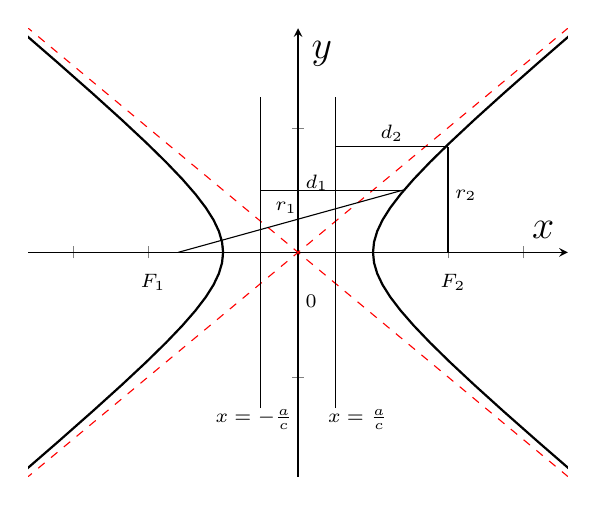
\begin{tikzpicture}[
every label/.style = {font=\tiny, inner sep=2pt, anchor=west},
        dot/.style = {circle, fill, inner sep = 1pt}
                        ]
    \begin{axis}[
        axis lines=middle,
        xlabel=$x$,
        ylabel=$y$,
        xmin=-3, xmax=3,
        ymin=-3, ymax=3,
        yticklabel=\\, xticklabel=\\,
        enlargelimits]
        \addplot [thick,domain=-2:2] ({cosh(x)}, {sinh(x)});
        \addplot [thick,domain=-2:2] ({-cosh(x)}, {sinh(x)});
        \addplot[red,dashed] expression {x};
        \addplot[red,dashed] expression {-x};
        \addplot[solid, draw = black] coordinates {(-0.5,-2.5) (-0.5,2.5)};
        \addplot[solid, draw = black] coordinates {(0.5,-2.5) (0.5,2.5)};
        \addplot[solid, draw = black] coordinates {(-1.6,0) (1.4, 1)};
        \addplot[solid, draw = black] coordinates {(-0.5,1) (1.4, 1)};
        \addplot[solid, draw = black] coordinates {(2,0) (2, 1.7)};
        \addplot[solid, draw = black] coordinates {(0.5,1.7) (2, 1.7)};
        \node[label=135:{0}] at (0.2,-1) {};
        \node[label=135:{$F_1$}] at (-2,-0.7) {};
        \node[label=135:{$F_2$}] at (2,-0.7) {};
        \node[label=135:{$x=-\frac{a}{c}$}] at (-1,-2.9) {};
        \node[label=135:{$x=\frac{a}{c}$}] at (0.5,-2.9) {};
        \node[label=135:{$r_1$}] at (-0.2,0.5) {};
        \node[label=135:{$r_2$}] at (2.2,0.7) {};
        \node[label=135:{$d_1$}] at (0.2,0.9) {};
        \node[label=135:{$d_2$}] at (1.2,1.7) {};
    \end{axis}
\end{tikzpicture}

Рис. 25
\end{center}

\newpage
Так же, как и для эллипса, имеет место утверждение: $\frac{r_1}{d_1}=\frac{r_2}{d_2}=e$, где $d_1$ и $d_2$ - расстояния от точки гиперболы до соответствующих директрис (рис. 25б). 
Доказательство совершенно аналогично тому, что проведено для эллипса,  и поэтому мы приводить его не будем. Приведем лишь формулировку теоремы, которая является фактически еще одним определением гиперболы:

\textit{Теорема.} Отношение растовния от любой тоики гиперболы до фокуса к расстоянию ее до соответствующеи директ рисы есть величина постоянная, равкая әксцект риситету гиперболы е $>1$.

Отметим, тто гипербола $\frac{y^2}{b^2}-\frac{x^2}{a^2}=1$ называется coпряженной по отношению к гнперболе (12.1). Действнтельной осью сопряженной гиперболы является ось $O y$, асимптоты остаются прежними.

Перейдем. к установлению геометрнческих свойств и вида формы параболы:
\[
y^2=2p x \hspace{10} (p>0) . \tag{12.6}\label{myeq}
\]


Прежде всего отметнм, что кривая лежит в правой полуплоскости ( $x \geqslant 0$ ) и проходнт через начало координат. Рассмотрим точку $F\left(\frac{p}{2} ; 0\right)$, называемую фокусом параболы, и прямую, перпендикулярную к оси $O x$, с уравнением $x=-\frac{p}{2}$, называемую директрисой пaраболы. Пусть $M(x ; y)$ - произвольная точка параболы. Вычислим расстоянне
$$
|\overrightarrow{F M}|=r=\sqrt{\left(x-\frac{p}{2}\right)^2+y^2},
$$

подставив $y^2$ из соотношения (12.6). Получим
\[
r=\sqrt{\left(x+\frac{p}{2}\right)^2}=\left|x+\frac{p}{2}\right|=x+\frac{p}{2} .\tag{12.7}\label{myeq}
\]

Расстояние $d$ от $M$ до днректрисы $x=-\frac{p}{2}$ также равно $x+\frac{p}{2}$. Поэтому для параболы $\frac{r}{d}=1$. Таким \newpage образом, парабола есть ГМТ, для которых расстояние до фиксированной точки $F$ (фокуса параболы) равно расстоянию до фиксированной прямой (директрисы параболы).

Так как для эллипса и гиперболы отношение $\frac{r}{d}$ есть постоянное число, равное $e$-эксцентриситету, то и для параболы отношенне $\frac{r}{d}=e$ называют эксцентриситетом, т.е. для параболы $e=1$.
Из приведенного рассуждения следует, что эллипс, гипербола н парабола обладают общим геометрическим свойством: отношение расстояния $r$ от любой точки $М$ каждой из этих кривых до фокуса к расстоянию $d$ от этой точки $M$ до соответствующей директрисы есть велична постоянная, равная эксцентриситету $е$ кривой.

Форма параболы легко устанавливается с использованием симметрии относительно оси $O x$ н монотонного возрастания функции $y=\sqrt{2 p x}$ (рис. 26a).
Для вывода единого уравнения эллипса, гигерболы и параболы в полярной системе координат воспользуемся установленным единным для этих кривых свойством $\frac{r}{d}=e$.

Пусть задана какая-либо нз перечисленных кривых. Поместим полюс полярной системы координат в фокус $F$, а полярную ось -- по перпендикуляру от директрисы к фокусу (рис. 26б).
Пусть $B$ - точка пересечения кривой с перпендикуляром к полярной оси, исходящим нз фокуса $F$, а $p$-- длина вектора $\overrightarrow{F B}$, называемая фокальным параметром. Согласно свойству $\frac{r}{d}=e$ имеем, что $\frac{p}{|\overrightarrow{C B}|}=$ $=\frac{p}{|\overrightarrow{E F}|}=\boldsymbol{e}$. Поэтому $|\overrightarrow{E F}|=\frac{p}{e}$, а также
$$
d=|\overrightarrow{D M}|:|\overrightarrow{E M}|^{\prime}=|\overrightarrow{E F}|+r \cos \varphi=\frac{p}{e}+r \cos \varphi .
$$

Подставляя данное выражение в отношенне $\frac{r}{d}=e$, получим

\newpage


\begin{center}
\begin{figure}
    \centering
    \includegraphics[width=0.8\linewidth]{Graf.png}    
\end{figure}
$\frac{r}{\frac{p}{e} + rcos\phi} = e$,
\end{center}

откуда следует полярное уравнение для рассматриваемых кривых второго порядка ($e<1$ - эллипс, $e>1$ - гипербола, $e=1$ - парабола):


\end{document}